\documentclass[times, 10pt,twocolumn]{article}

\usepackage{sose2011}
\usepackage{times}
\usepackage[pdftex]{graphicx}

\graphicspath{{./images/}}
\DeclareGraphicsExtensions{.pdf,.jpeg,.png,.jpg}

% correct bad hyphenation here
\hyphenation{op-tical net-works semi-conduc-tor}
\pagestyle{empty}

\begin{document}

\title{Managed Control of Composite Cloud Systems}

\author{
        \textbf{Christopher Lamb}\hspace*{0.3in}
        \textbf{Pramod Jamkhedkar}\hspace*{0.3in}
        \textbf{Greg Heileman}\\
        Department of Electrical and Computer Engineering \\
        University of New Mexico \\
        \small{\{cclamb, pramod54, heileman\}@ece.unm.edu}
}

\maketitle
\thispagestyle{empty}

\begin{abstract}
Cloud providers have just begun to provide primitive functionality enabling users to configure and easily provision resources, and primarily in the Infrastructure as a service domain at that.  In order to effectively manage cloud resources in an automated fashion, systems must automate quality of service metric measurement as a part of a larger usage management strategy.  Collected metrics can then be used within control loops to manage and provision cloud resources when needed.  This basic approach can be scaled to monitor the use of system artifacts as well as simple quality-of-service parameters, and can also address the needs of large systems spanning the boundaries of single service providers.
\end{abstract}

{
\setlength{\parindent}{0mm}
\textbf{Keywords:} Usage Management, Cloud Computing, System of Systems.
}

\section{Introduction}
Cloud computing services as a computational paradigm are more market oriented than previous attempts at commodity computing.  Furthermore, they are in many cases designed to be composed into larger, more powerful customer facing systems.  These kinds of aggregate systems fit neatly into one of the more commonly used definitions of a system of systems as well \cite{Sose:SageCuppan:2001}, \cite{Sose:Web:Defns}.  With so much data in the hands of different providers in an aggregate system, system developers and users are hard-pressed to effectively monitor and control the use of sensitive content by various composite systems.  Some of this information can be contained in Service Level Agreements (SLAs), but they have thus far been focused on quality-of-service (QoS) metrics rather than addressing issues like data flow or physical application residency.  For the most part SLAs are simply not sufficient for addressing usage management concerns \cite{WSA}, \cite{WSLA}, \cite{WSP}, \cite{PaRaSh:09}.

Effective usage management monitoring coupled with feedback processing creates an event loop suitable for applying control theoretic concepts to cloud infrastructures.

Usage policies specified at a fine-grained level provides cloud service users with more reliability of the use of their data within cloud centric systems.  For example, data routing, caching, or hosting can be a sensitive issue for some systems in that specific users may want to restrict the countries that can access that data.  The ability to specify and control where specifically that data travels and resides gives those kinds of sensitive users confidence to use could-centric computing resources.  Furthermore, this kind of control will also facilitate cost profiles for services that more closely match demand, giving providers better control over their infrastructure and additional areas for product differentiation.

Herein, we will elaborate the idea of applying usage management to single and distributed could systems.  In this brief analysis, we will touch on the application of common system design principles and standards \cite{BlCl:01}, \cite{Cl:88}, \cite{ClWrSoBr:02}, application of usage control concepts \cite{PaSa:04}, \cite{JaHeLa:10}, policy language application \cite{JaHeMa:06}, digital rights management (DRM) systems~\cite{JaHe:09}, and interoperability~\cite{JaHe:04}, \cite{HeJa:05}, \cite{KoLaMaMi:04}, \cite{coral}, \cite{marlin}.  We will apply these ideas toward a controllable feedback-enabled system suitable for cloud system control.

In Section~\ref{sec:single} this paper first addresses how to create a controllable system with feedback suitable for system evaluation from the perspective of a single provider. Here, we will address the constraints and advantages of such an approach and how providers could begin to offer these kinds of services.  In this first example, we will focus on QoS data specifically.  Next in Section~\ref{sec:singleUm} we will extend our single provider system to provide control over attributes more specific to the usage management domain, with examples and associated analysis.  Finally in Section~\ref{sec:multiple} we extend this single provider model to a more realistic system deployed to multiple cloud providers in a realistic system-of-systems scenario.

\subsection{Previous Work}
In the recent years, cloud computing has  managed to emerge as a computing platform that allows computing services to be consumed as a utility by consumers. In cloud computing, applications, systems software, and hardware are offered as utility services to consumers over the Internet. In service-based architectures, service consumers need to be provided with  highly reliable services that meets their expectations. The consumers indicate these expectations in terms of QoS parameters that are expressed in the form of an SLA negotiated with the service provider. 

In the realm of computing, there exist multiple service-based paradigms such as web-services, cluster computing, grid computing and cloud computing~\cite{Bu:09}. Cloud computing is set apart from the other forms of service-based computing paradigms by  the collective set of distinguishing characteristics such as market orientation, visualization, dynamic provisioning of resources and service composition via multiple service providers~\cite{BuYeVeBrBr:09}. These characteristics imply that in cloud computing, data and application of a cloud-service consumer reside inside the cloud for a finite amount of time; fractions of this data are handled by multiple cloud services; and these data fractions may be stored, processed and routed across a geographically distributed cloud infrastructure. These activities occur ``behind-the-scenes'', within the cloud, while giving the cloud consumer an impression of a single virtual machine. These operational characteristics of cloud computing raise serious  concerns regarding the manner in which data and application of cloud consumers are handled or used within the cloud. Unlike other computing paradigms that focus on specific computing tasks, cloud computing enables cloud consumers to host entire applications on the cloud. As consumers aggressively start exploiting this advantage to ``outsource'' their IT services to the cloud, the manner in which data and application is handled within the cloud by various cloud services will become a matter of serious concern.  

The handling or use of consumer data within the cloud by different services refers to the policies regarding constraints under which different actions may be carried out on the data. A cloud consumer might want to limit the way in which data is stored, routed, or processed, and specify who is authorized to carry out these activities and under what conditions. As an example, a government agency might want to prevent the data from being stored in one particular country, or prevent the routing of its data via a particular set of networks it considers unreliable. Similarly, a financial company might want to prevent its data from being processed by a particular cloud service, or may want it to be encrypted before being stored by an untrusted cloud storage service. Usage policies typically consists of a range of semantics such as restrictions on the manner in which data is used, temporal restrictions on usage, spacial or attribute-based restrictions, permissions, obligations, penalties, count-based limits on usage and partial dependencies to name a few.   Hence, as cloud services become pervasive, cloud consumers will want to dictate the terms of usage for their data and applications within the cloud in a manner that is expressive enough to capture the concerns of cloud users. At present, cloud providers enable these features via rudimentary techniques by offering a one-size-fits-all options to consumers. For example, Amazon S3 storage services allow a region-based facility where data stored in one region is guaranteed not to leave that particular region~\cite{AWS}. Future cloud computing services will need to enable these terms to be expressed in SLAs in a sophisticated, fine-grained manner that will allow the cloud consumers to express the usage terms explicitly. 

As mentioned earlier, service expectations in service-based computing paradigms are expressed in terms of SLAs negotiated with the service provider. For different types of service-based computing paradigms such as web services, clusters, and grid computing, there exist well established SLA frameworks that enable expression, interpretation, monitoring, control and enforcement of SLA terms~\cite{WSA, WSLA, WSP,PaRaSh:09}. However, the SLAs supported by these frameworks focus on performance metrics such as availability, reliability, bandwidth, response times, instructions per second, etc. ~\cite{PaSc:06}. Also, the privacy and security metrics supported by these frameworks focus primarily on encryption of the data. It must be noted that usage policies are significantly different than these metrics and present a new dimension that is orthogonal to the manner in which the other metrics are managed. It is therefore necessary to have a separate mechanism for usage management in cloud computing environments. The next section discusses the characteristic features of such a framework.


%\begin{figure}[!t]
%\centering
%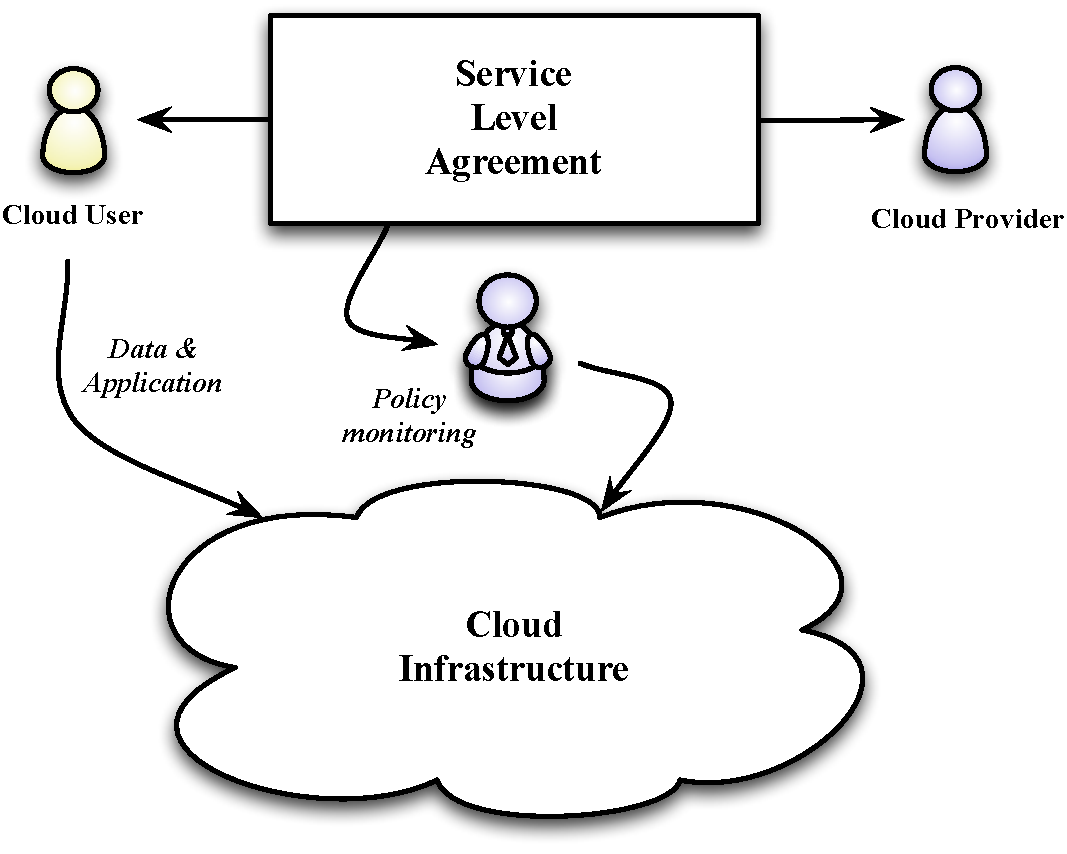
\includegraphics[width=3in]{Overview.pdf}
%\caption{Overview of the manner in which SLAs are implemented in present cloud environments.}
%\label{fig:overview}
%\end{figure}

%\cite{Emr:Web:Jade,Emr:Web:Fipa}.
%\cite{KoLaMaMi:04,SaShUe:04}

\section{Single Provider Feedback System}\label{sec:single}

\section{Single Provider Feedback System with Usage Management}\label{sec:singleUm}

\section{Scaling to Multiple Providers}\label{sec:multiple}

\section{Conclusion}
In this paper we introduced the notion of usage management in cloud computing environment. Cloud computing exhibits a unique set of characteristics that will require usage management of users' data according to user concerns and expectations. We analyzed the challenges involved in the design and development of a framework for usage management in cloud environments. We showed that such a framework needs to be open to leverage existing security technologies and SLA frameworks. The framework needs to exhibit features such as support for multiple policy languages, existence of a common cloud ontology, dynamic interpretation and data transformations. Finally a preliminary framework that supports multiple policy languages was introduced that will provide a platform upon which such a framework can be built. 

Future works involves efforts towards the development of a common extensible cloud ontology that will provide the vocabulary underlying this framework and enable interoperability. Such an ontology needs be developed by taking into consideration the requirements of different cloud services. In addition, it is necessary to standardize interfaces for other security mechanisms mentioned in the paper that can be incorporated within the framework. Finally, the framework allows use of multiple policy languages, to this effect, existing policy languages can be modified to be incorporated within the framework, and news ones need to designed to address the specific needs of different cloud services.

\bibliographystyle{IEEEtran}
\bibliography{emr,drm,sose}

\end{document}


